%!TEX root = main.tex
\section{Central diffraction}

\begin{frame}
\frametitle{Central diffraction study}

\begin{itemize}
	\item{$f_0(980)$, $f_2(1270)$ and $f_0(1500)$ are controversial}
	\begin{itemize}
		\item $q\bar{q}$ ?
		\item or gg (glueball) ?
		\item or $q\bar{q}g$ (hybrid)?
	\end{itemize}
	\item{Central diffraction at LHC energy level}
	\begin{itemize}
		\item Double-pomeron exchange dominates
		\item Pomeron is the leading order of a gluon pair
		\item A good environment for glueballs and hybrids
	\end{itemize}
	\item{main goals}
	\begin{itemize}
		\item Fix spin of resonances in CD events with the PWA
		\item PWA test with well known $f_0(980)$, $f_2(1270)$ 
		\item Apply PWA to other resonances and check if they have a exotic spin number
	\end{itemize}
	
\end{itemize}

\end{frame}

\begin{frame}[c]
\frametitle{Partial wave dissociation}
\begin{columns}[c]
\column{.5\textwidth}
\includegraphics[width=1.\linewidth]{data2pion}
\column{.5\textwidth}
\tiny
\begin{itemize}
\item Collecting CD events by Double-Rapidity Gaps
\item Double Pomeron Exchange confines the system with $\mathrm{J}^{PC} = 0^{++}, 2^{++}...$
\item $f_0(980) ( 0^{++})$, $f_2(1270) ( 2^{++})$ get dominated
\item $\rho_0(770) ( 1^{- -})$, $K^0_{S} ( 0^{-})$ get suffressed
\item Partial Wave Decomposition for S ($f_0(980)$) and D ($f_2(1270)$) waves 
\end{itemize}
\end{columns}
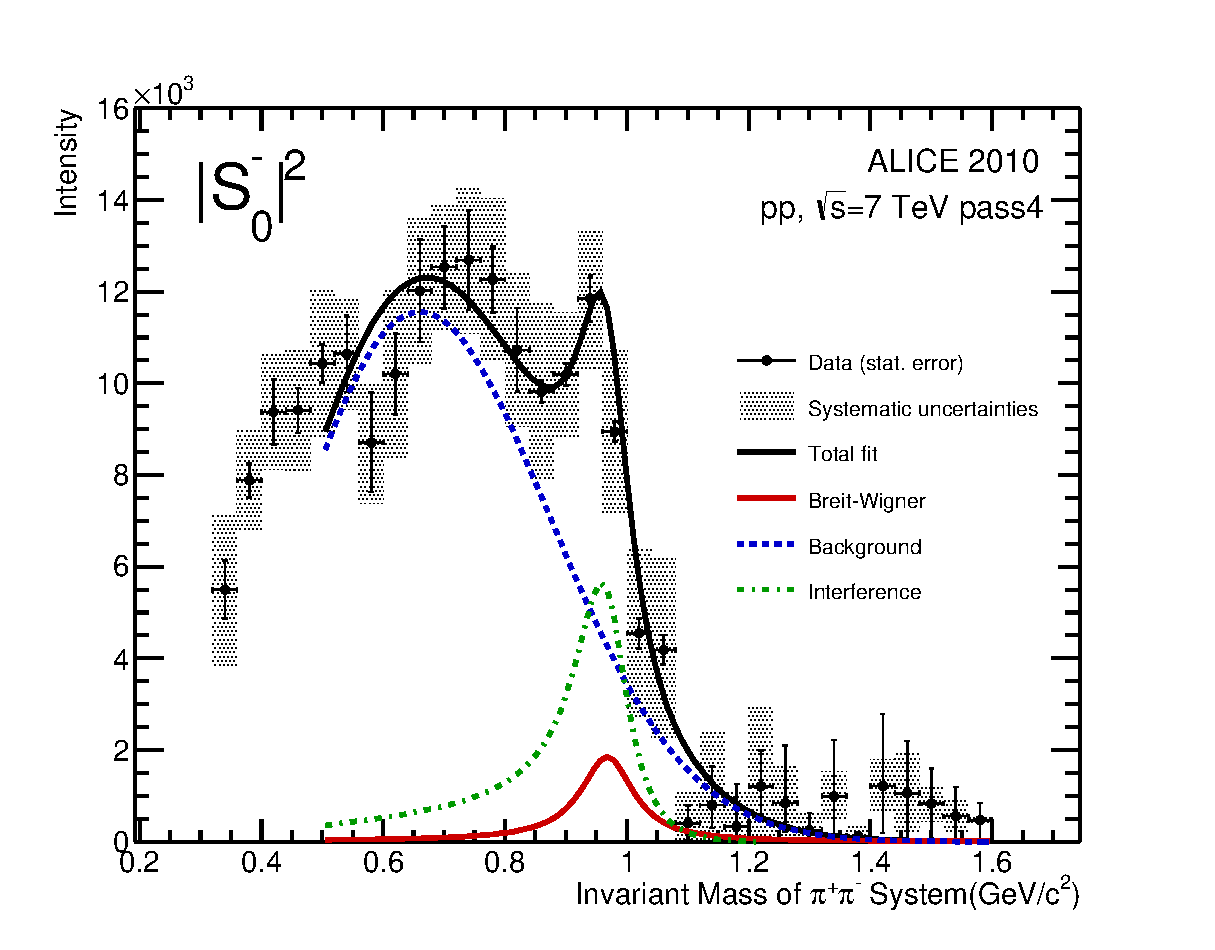
\includegraphics[width=0.5\linewidth]{c_s0_fit_kps}
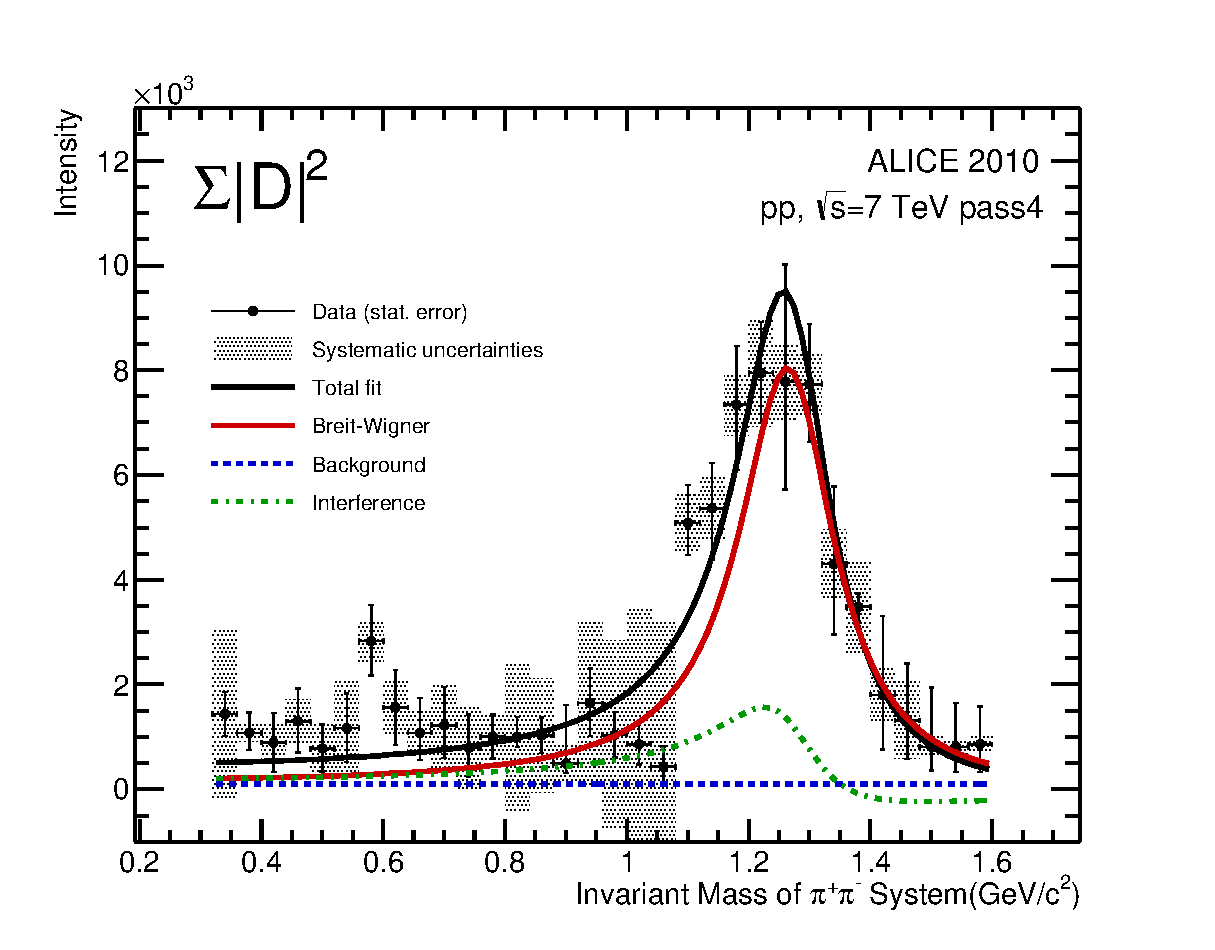
\includegraphics[width=0.5\linewidth]{c_d0_fit_kps}
\end{frame}



